\chapter{Diseño e Implementación} % Main chapter title

\label{Chapter3} % Change X to a consecutive number; for referencing this chapter elsewhere, use \ref{ChapterX}
\definecolor{mygreen}{rgb}{0,0.6,0}
\definecolor{mygray}{rgb}{0.5,0.5,0.5}
\definecolor{mymauve}{rgb}{0.58,0,0.82}

\lstset{ %
  backgroundcolor=\color{white},   % choose the background color; you must add \usepackage{color} or \usepackage{xcolor}
  basicstyle=\footnotesize,        % the size of the fonts that are used for the code
  breakatwhitespace=false,         % sets if automatic breaks should only happen at whitespace
  breaklines=true,                 % sets automatic line breaking
  captionpos=b,                    % sets the caption-position to bottom
  commentstyle=\color{mygreen},    % comment style
  deletekeywords={...},            % if you want to delete keywords from the given language
  %escapeinside={\%*}{*)},          % if you want to add LaTeX within your code
  %extendedchars=true,              % lets you use non-ASCII characters; for 8-bits encodings only, does not work with UTF-8
  %frame=single,	                   % adds a frame around the code
  keepspaces=true,                 % keeps spaces in text, useful for keeping indentation of code (possibly needs columns=flexible)
  keywordstyle=\color{blue},       % keyword style
  language=[ANSI]C,					% the language of the code
  %otherkeywords={*,...},           % if you want to add more keywords to the set
  numbers=left,                    % where to put the line-numbers; possible values are (none, left, right)
  numbersep=5pt,                   % how far the line-numbers are from the code
  numberstyle=\tiny\color{mygray}, % the style that is used for the line-numbers
  rulecolor=\color{black},         % if not set, the frame-color may be changed on line-breaks within not-black text (e.g. comments (green here))
  showspaces=false,                % show spaces everywhere adding particular underscores; it overrides 'showstringspaces'
  showstringspaces=false,          % underline spaces within strings only
  showtabs=false,                  % show tabs within strings adding particular underscores
  stepnumber=1,                    % the step between two line-numbers. If it's 1, each line will be numbered
  stringstyle=\color{mymauve},     % string literal style
  tabsize=2,	                   % sets default tabsize to 2 spaces
  title=\lstname,                   % show the filename of files included with \lstinputlisting; also try caption instead of title
  morecomment=[s]{/*}{*/}%
}

En este capítulo se presentan la arquitectura multicore del firmware, los mecanismos de comunicación entre procesadores y el detalle del diseño de los módulos desarrollados junto con sus interfaces.

%----------------------------------------------------------------------------------------
%	SECTION 1
%----------------------------------------------------------------------------------------

\section{Arquitectura multicore}
\label{sec:arquitectura}

El \textit{firmware} está desarrollado sobre la base de dos proyectos vinculados del IDE MCUXpresso, uno para cada \textit{core} del microcontrolador. Para el IDE, debe haber un proyecto ``maestro'' que controle la ejecución del código (o al menos la secuencia de \textit{startup}) corriendo en el otro \textit{core}, considerado ``esclavo''.  

El proyecto maestro contiene un link al proyecto esclavo que produce que la imagen binaria del esclavo sea incluida en la imagen  binaria del maestro, cuando el proyecto maestro es compilado \citep{nxp:mcuxpresso}. De esta manera, cuando el proyecto maestro es grabado en la flash del microcontrolador, ambos proyectos son descargados a la memoria del microcontrolador.

El proyecto maestro debe ser el que se ejecuta sobre el procesador Cortex-M4 ya que el procesador Cortex-M0 permanece en estado de \textit{reset} hasta que el otro core lo libera de este estado escribiendo un 0 en el bit M0SUB\_RST del registro RESET\_CTRL1, como se indica en el manual del microcontrolador \citep{nxp:lpc4337}.

Cuando se energiza el microcontrolador o se produce un \textit{reset}, el \textit{core} maestro inicia su secuencia de \textit{startup} y es responsable de iniciar, a su vez, la secuencia de \textit{startup} del \textit{core} esclavo.  

En las tablas \ref{tab:memoriaM4} y \ref{tab:memoriaM0} se muestra la asignación de bloques de memoria para los procesadores Cortex-M4 y Cortex-M0, respectivamente.  Puede verse que el código de cada procesador se ubica en un bloque de memoria flash independiente, los bancos A y B de 512 kB cada uno.  

Por otra parte, para evitar cualquier tipo de solapamiento en el uso de la RAM, los proyectos asociados a cada \textit{core} se linkean de forma de utilizar exclusivamente bancos de RAM separados.  En este sentido, el procesador cortex-M4 utiliza el primer bloque de RAM de 32 kB y el procesador cortex-M0 utiliza el segundo bloque de RAM de 40kB.

\begin{table}[ht]
\caption{Asignación de bloques de memoria para el Cortex-M4}
\begin{tabular}{lllll}
\toprule
\textbf{Tipo de memoria} & \textbf{Nombre} & \textbf{Alias} & \textbf{Ubicación} & \textbf{Tamaño} \\ 
\midrule
Flash                    & MFlashA512      & Flash          & 0x1a000000         & 0x80000         \\
RAM                      & RamLoc32        & RAM            & 0x10000000         & 0x8000          \\ 
\bottomrule
\end{tabular}
\label{tab:memoriaM4}
\end{table}

\begin{table}[ht]
\caption{Asignación de bloques de memoria para el Cortex-M0}
\begin{tabular}{lllll}
\toprule
\textbf{Tipo de memoria} & \textbf{Nombre} & \textbf{Alias} & \textbf{Ubicación} & \textbf{Tamaño} \\ 
\midrule
Flash                    & MFlashB512      & Flash2          & 0x1b000000         & 0x80000         \\
RAM                      & RamLoc40        & RAM2            & 0x10080000         & 0xa000          \\ 
\bottomrule
\end{tabular}
\label{tab:memoriaM0}
\end{table}

Adicionalmente, se define una zona de memoria compartida, visible por ambos procesadores para el intercambio de información. Los mecanismos de comunicación inter-procesadores (IPC, del inglés \textit{Inter Processor Communication}) se describen en la sección \ref{subsec:IPC}. 

\begin{verbatim}
/* Shared memory used by IPC */
#define SHARED_MEM_IPC   0x10088000	 
\end{verbatim}

\subsection{Inter Processor Communications}
\label{subsec:IPC}

Para comunicar ambos procesadores se utiliza una biblioteca provista por el fabricante del microcontrolador NXP, documentada en la nota de aplicación ``AN1117: Inter Processor Communications for LPC43xx'' \citep{nxp:an1117}. En este documento se explican 3 mecanismos posibles para que los dos procesadores intercambien información basados en interrupciones, en colas de mensajes y en ``casillas de correo''.  Este útltimo método queda excluido de esta memoria por no haber sido utilizado en el desarrollo.

\subsubsection{Interrupción}

El mecanismo de interrupciones cruzadas es el más simple de los 3 métodos provistos.  Permite que un \textit{core} active una interrupción en el otro \textit{core} para enviar notificaciones cuya interpretación depende y es exclusiva de la aplicación.  El diseñador puede definir una función de \textit{callback} que es ejecutada en el contexto de la rutina de servicio de la interrupción.  

Para enviar señales al \textit{core} ``remoto'', el \textit{core} ``local'' utiliza una instrucción dedicada SEV (\textit{send event}) provista por la arquitectura Cortex.  

Asimismo, dentro de la rutina de interrupción se habilita un \textit{flag} para indicar que se ha recibido una notificación IPC.  Esta variable \textit{flag} puede ser usada por las aplicaciones corriendo sobre el \textit{core} que recibe la notificación para chequear el estado de las comunicaciones. La limpieza del \textit{flag} se hace dentro de una sección crítica donde se deshabilitan temporalmente las interrupciones.  En el Cortex-M4 se enmascaran las interrupciones con mayor prioridad y en el Cortex-M0 se deshabilitan directamente ya que este procesador no dispone del mecanismo de enmascaramiento.

\subsubsection{Colas de mensajes}

En el método de la cola de mensajes, el diseñador define dos áreas de memoria compartida, que se utilizan para almacenar los mensajes que cada procesador envía al otro. Un búfer de comandos del \textit{host} está dedicado a los comandos enviados del maestro al esclavo, y un búfer de mensajes del \textit{host} se dedica a los mensajes que el esclavo envía en respuesta. La figura \ref{fig:IPC} muestra la configuración.

\begin{figure}[ht]
	\centering
	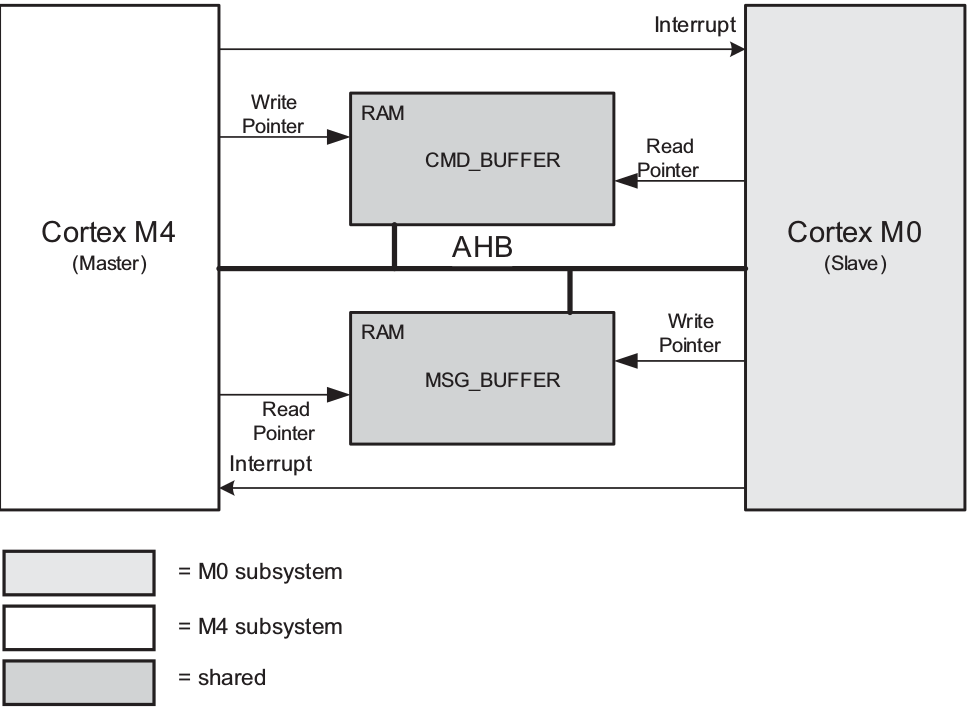
\includegraphics[width=.8\textwidth]{./Figures/IPC.png}
	\caption[Esquema de comunicación entre procesadores]{Esquema de comunicación entre procesadores basado en colas de mensajes\protect\footnotemark.}
	\label{fig:IPC}
\end{figure}

\footnotetext{Imagen tomada del manual de usuario del microcontrolador LPC4337 \citep{nxp:lpc4337}}

\section{Diseño de módulos y definición de interfaces}
\label{sec:modulos}

\section{Módulo de almacenamiento}
\label{sec:almacenamiento}

\section{Módulo de adquisición}
\label{sec:adquisicion}

\subsection{Sensor de temperatura}
\label{subsec:1-wire}

\subsection{Sensor de velocidad de viento}
\label{subsec:anemometro}

\section{Módulo interfaz HMI}
\label{sec:HMI}

\section{Módulo de control}
\label{control}
